\subsection{Schwache Kopplung und starke Kohäsion}
\label{sec:Kap-9.1.2}

Zur Minimierung von Komplexität sollte jedes Modul nur eine Aufgabe erfüllen. Gleichzeitig sollten zwischen Modulen nur wenige, einfache Beziehungen existieren. Auf diese Weise werden Anpassungen am Quellcode bei gewünschten Änderungen auf wenige Module begrenzt und die Wiederverwendbarkeit der einzelnen Module erhöht. Man formuliert diesen Idealzustand als „schwache Kopplung und starke Kohäsion“.

Die \textit{Kohäsion} 
\marginline{Kohäsion betrifft einzelne Klassen}
gibt an, wie eng die Teile einer Klasse (z.B. verschiedene Attribute und Operationen) logisch zusammenhängen. Starke Kohäsion ist dann gegeben, wenn es einen engen Bezug zwischen allen Teilen einer Klasse gibt. In diesem Fall erfüllt eine Klasse genau eine Aufgabe und alle Teile der Klasse tragen zur Erfüllung genau dieser Aufgabe bei. 

Die \textit{Kopplung} 
\marginline{Kopplung betrifft Beziehungen zwischen Klassen}
ist ein Maß für die Komplexität der Beziehungen zwischen Klassen. Starke Kopplung besteht, wenn für die Erfüllung einer Aufgabe viele Klassen zusammenarbeiten müssen und somit viele Abhängigkeiten zwischen den Klassen bestehen. Zwei Klassen \sttpUMLText{A} und \sttpUMLText{B} sind beispielsweise gekoppelt, wenn die Instanzen der Klasse \sttpUMLText{A} als Dienstnutzer von Instanzen der Klasse \sttpUMLText{B} (und damit Instanzen von \sttpUMLText{B} als Dienstleister für Instanzen von \sttpUMLText{A}) auftreten oder umgekehrt. Typischerweise werden dabei vom Dienstnutzer Nachrichten an den Dienstleister über Verbindungen gesendet, die als Assoziationen zwischen den Klassen modelliert sind. Allgemein formuliert sind zwei Klassen gekoppelt, wenn 

\begin{itemize}
	\item es eine Assoziation zwischen den Klassen gibt,
	\item der Datentyp einer Klasse als Parametertyp in einer Operation der anderen Klasse aufritt,
	\item Instanzen einer Klasse in einer Operation der anderen Klasse erzeugt werden oder
	\item zwischen den Klassen eine Generalisierungsbeziehung existiert.
\end{itemize}

Starke Kohäsion und schwache Kopplung sind leider häufig konkurrierend zueinander: Je stärker unterschiedliche Funktionalitäten auf unterschiedliche Klassen aufgeteilt werden (und damit die Kohäsion einer einzelnen Klassen hoch gehalten wird), desto mehr müssen einzelne Klassen für die Erfüllung ihrer Aufgabe auf Funktionalitäten anderer Klassen zugreifen (und damit wird auch die Kopplung zwischen den Klassen erhöht): Mit zunehmender Klassenzahl, also abnehmender Klassengröße, in einem Programm\-code steigt die Kohäsion, weil dann jede Klasse nur eine eng umrissene Aufgabe erfüllt. Andererseits nimmt aber auch die Kopplung zu. Der Umfang der Schnittstellen wächst, weil Operationen, die bei größeren Klassen nur innerhalb dieser bekannt waren, jetzt zwecks Weiterverarbeitung über die Schnittstellen auch anderen Klassen bekannt gemacht werden müssen.

Für die Praxis können aus diesen Überlegungen zwei Schlussfolgerungen gezogen werden:

\begin{enumerate}
	\item Zerlegt ein Entwurf ein Softwaresystem in zu wenige Klassen, so ist oft der logische Zusammenhang innerhalb der Klassen schwach. Die einzelnen Klassen sind groß und unübersichtlich, mit negativen Auswirkungen auf die Wartbarkeit und Wiederverwendbarkeit.
	\item Zerlegt ein Entwurf ein Softwaresystem in zu viele Klassen, so wird das 
	\linebreak %%% für Druck
	Beziehungsgeflecht aufgebläht. Dabei werden Details, die eigentlich innerhalb von Klassen verborgen bleiben könnten und sollten, über Schnittstellen nach außen gegeben und damit letztlich auch das Geheimnisprinzip untergraben.
\end{enumerate}

Es gibt Heuristiken, die dazu beitragen, die Kopplung abzuschwächen und es gibt Heuristiken, die helfen, die Kohäsion zu verstärken. Aufgrund der Konkurrenz-
\linebreak %%% für Druck 
situation der beiden Maße muss man bei deren Anwendung immer darauf achten, den jeweiligen Gegenpart nicht über Gebühr negativ zu beeinflussen. Einige Entwurfs\-muster (s.~Kap.~\ref{sec:Kap-10}) adressieren genau dieses Problem.

\minisec{Abschwächung der Kopplung}

Das grundsätzliche Ziel der Kopplungsabschwächung ist, dass Instanzen einer Klasse so wenig wie möglich mit Instanzen anderer Klassen zusammenarbeiten, \dasHeisst Verbindungen besitzen bzw. eingehen oder Nachrichten senden. \marginline{schmale Schnittstellen} Unterstützt wird diese Maxime durch schmale Schnittstellen: Die Anzahl der öffentlichen Operationen einer Klasse sollte so klein sein, dass gerade noch die Dienstnutzer befriedigt werden und so viel Interna wie möglich verborgen bleiben.

\pagebreak
Eine andere 
\marginline{Vermittlerklasse}
Möglichkeit, eine starke Kopplung (mehrerer) Klassen aufzubrechen, besteht in der Einführung einer vermittelnden Klasse, deren einzige Instanz sämtliche Dienstnutzungen zwischen den Instanzen der stark gekoppelten Klassen abwickelt. Abbildung~\ref{fig:kopplung_stark} zeigt ein Klassendiagramm, in dem eine starke Kopplung der Klassen \sttpUMLText{B}, \sttpUMLText{C}, \sttpUMLText{D} und \sttpUMLText{E} zu erkennen ist.

\begin{figure}[h!]
	\centering
	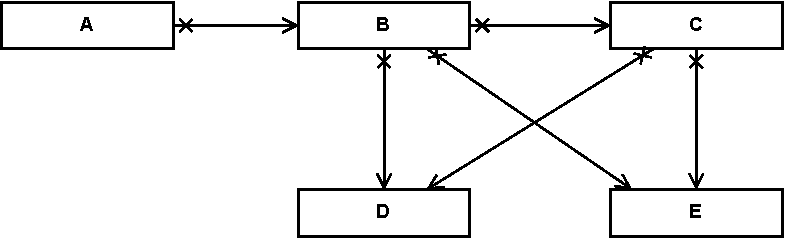
\includegraphics[scale=1.0]{Bilder/Kapitel-9/kopplung_stark.pdf}
	\caption{Stark gekoppelte Klassen \sttpUMLText{B}, \sttpUMLText{C}, \sttpUMLText{D} und \sttpUMLText{E}}
	\label{fig:kopplung_stark}
\end{figure}

Die Kopplung lässt sich mit einer Klasse \sttpUMLText{Vermittler} abschwächen, deren Instanz die Dienstleistungen der Instanzen der Klassen \sttpUMLText{D} und \sttpUMLText{E} gegenüber den Instanzen der Klassen \sttpUMLText{B} und \sttpUMLText{C} übernimmt. Tatsächlich reicht die Vermittlerklasse die Funktionalitäten der Klasse \sttpUMLText{D} und \sttpUMLText{E} nur durch. Abb.~\ref{fig:kopplung_abgeschwaecht} zeigt die Verwendung der Vermittlerklasse. \sttpUMLText{B} und \sttpUMLText{C} sind jeweils nicht mehr direkt mit \sttpUMLText{D} und \sttpUMLText{E}, sondern nur noch mit \sttpUMLText{Vermittler} gekoppelt. Lediglich der Vermittler kennt die Aufteilung der Beziehungen auf \sttpUMLText{D} und \sttpUMLText{E}, aber nicht mehr die Klassen \sttpUMLText{B} und \sttpUMLText{C}, die nur noch \sttpUMLText{Vermittler} kennen. Wird die Schnittstelle von \sttpUMLText{D} oder \sttpUMLText{E} geändert, wirkt sich die Änderung nur auf die Klasse \sttpUMLText{Vermittler}, aber nicht auf die Klassen \sttpUMLText{B} und \sttpUMLText{C} aus.

\begin{figure}[h!]
	\centering
	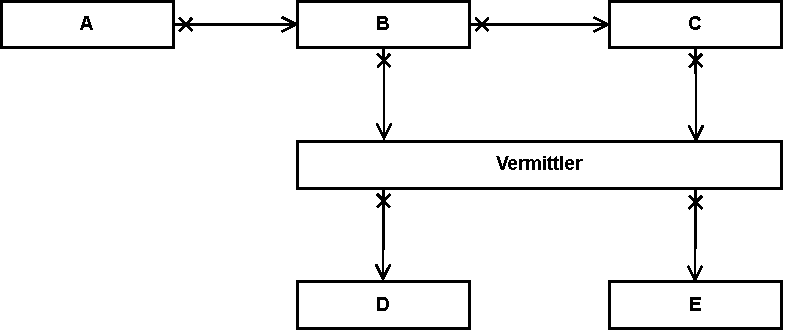
\includegraphics[scale=1.0]{Bilder/Kapitel-9/kopplung_abgeschwaecht.pdf}
	\caption[Abschwächung der Kopplung durch Vermittlerklasse]{Abschwächung der Kopplung durch Einfügen einer Vermittlerklasse}
	\label{fig:kopplung_abgeschwaecht}
\end{figure}

\pagebreak %%% für Druck

Eine dritte Variante zur Kopplungsabschwächung besteht darin, Funktionalität, welche eine Kopplung verursacht, in eine andere Klasse zu verschieben. Hier muss man im konkreten Fall aber prüfen, ob durch dieses Verschieben Kopplung an anderer Stelle erhöht wird, das Problem also nur verlagert wird. Gleichzeitig kann eine solche Maßnahme auch die Kohäsion der Klasse, in die die Funktionalität verschoben wird, schwächen.

In Aggregations- und Kompositionsbeziehungen lässt sich Kopplung abschwächen, indem nur die Ganzes-Klasse ihre Teile kennt, aber nicht umgekehrt, und indem sich zudem die unterschiedlichen Instanzen der Teile-Klasse nicht gegenseitig benutzen.

Eine 
\marginline{Law of Demeter} als „Law of Demeter“\footnote{Demeter ist hier weder Name eines Informatikers oder einer Informatikerin noch ein Bio-Anbauverband, sondern eine griechische Göttin, die dieses Prinzip aber wohl auch nicht erfunden hat.} bekannte Heuristik begrenzt die erlaubten Dienstleister auf der Ebene von Operationsaufrufen. Die Heuristik verhindert insbesondere, dass ein Objekt durch Navigation über mehrere Objektverbindungen hinweg Operationen von Klassen aufruft, die nicht direkt mit seiner Klasse assoziiert sind:

In einer Operation \sttpUMLText{o()} einer Klasse \sttpUMLText{K} sollten nur Operationen folgender Klassen benutzt werden.

\begin{itemize}
	\item \sttpUMLText{K} selbst,
	\item Klassen, die als Parametertypen von \sttpUMLText{o()} vorkommen,
	\item mit \sttpUMLText{K} assoziierte Klassen und
	\item Klassen, von denen bei der Ausführung von \sttpUMLText{o()} Instanzen erzeugt werden.
\end{itemize}

Bei konsequenter Anwendung dieser Heuristik ist es oft erforderlich, dass eine Klasse Operationen von mit ihr assoziierten Klassen in ihrer eigenen Schnittstelle anbietet und somit eine Art Vermittlerrolle spielt.

\minisec{Verstärkung der Kohäsion}

Eine zu schwache Kohäsion eines Moduls kann man grundsätzlich durch Zerlegung des Moduls in kleinere Module beheben (bei Begrenzung der negativen Auswirkungen auf die Kopplung). Aber woran erkennt man eine zu schwache Kohäsion einer Klasse? Eine oftmals zutreffende Heuristik dazu ist:

\begin{itemize}
	\item Lassen sich die Attribute und die Operationen einer Klasse in (weitgehend) disjunkte Teilmengen zerlegen, so dass jede Operationsmenge nur auf jeweils einer Attributmenge arbeitet, dann ist die entsprechende Aufteilung der Klasse zu empfehlen.
\end{itemize}

Die Anwendung der Heuristik ist umso sinnvoller, je kleiner die jeweiligen Durchschnitte der Attribut- und Operationsmengen sind. Lassen sich keine weitgehend disjunkten Teilmengen der Attribute und Operationen finden, liegt ein starkes Indiz dafür vor, dass die Kohäsion der Klasse stark genug ist.

Kohäsion ist im Übrigen ein Maß, das nicht nur auf Klassen (oder größere Module), sondern auch auf einzelne Operationen anwendbar ist. Eine Operation besitzt eine starke Kohäsion, wenn sie eine einzige, eng umrissene und klar abgegrenzte Funktionalität erbringt.